\subsection{Motivation}

\begin{frame}
  \frametitle{Reactor systems potentially meeting the Generation IV goals}
               \begin{figure}[t]
                \vspace*{-0.1in}
                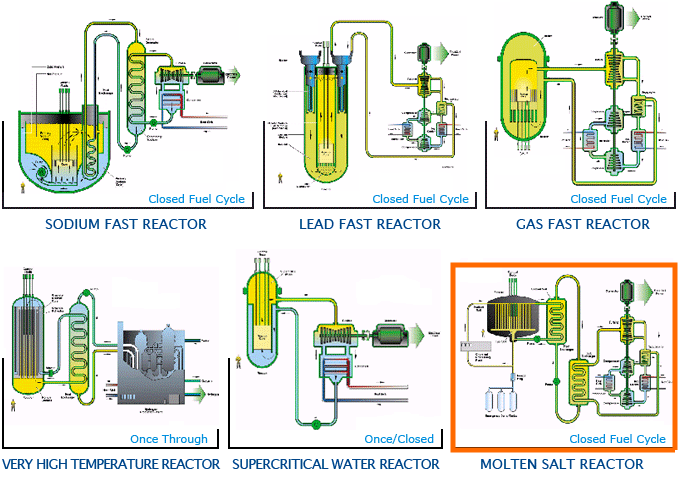
\includegraphics[height=0.65\textwidth]{./images/6_types.png}
                 \caption{Potential Generation IV reactors \cite{ABRAM2008}.}
               \end{figure}
              
\end{frame}

\begin{frame}
  \frametitle{Why Molten Salt Reactors?}
                  \vspace*{-0.1in}
              \begin{block}{Main advantages of liquid-fueled \glspl{MSR}}
               \begin{enumerate}
               \item High average coolant temperature (600-750$^{\circ}$C) $\Rightarrow$ high thermal efficiency, hydrogen production, cheap heat for chemical industry.
                \item May operate with epithermal or fast neutron spectrums.
                \item Various fuels ($^{235}$U, $^{233}$U, Thorium, U/Pu).
                \item Inherent safety advantages: fuel already liquid and drains into tanks in emergency.
                \item Large fuel utilization $\Rightarrow$ less nuclear waste generated.
                \item Online reprocessing and refueling.
               \end{enumerate}
               \end{block}
               
               \begin{block}{Main advantages of \gls{MSBR}}
               \begin{enumerate}
                \item Breed fissile $^{233}$U from $^{232}$Th with the breeding ratio 1.06 gives an annual 
                fissile yield of 3.3\%.
                \item Fuel salt heats up to 705$^{\circ}$C which makes thermal efficiency of over 44\%.
                \item $^{233}$U, $^{235}$U, or $^{239}$Pu could be used for the initial fissile loading.
                \item Outstanding neutron economy because of single-fluid two-region design.
               \end{enumerate}
               \end{block}

\end{frame}

\begin{frame}
  \frametitle{Molten Salt Reactor Experiment vs Molten Salt Breeder Reactor}
  \begin{columns}
    \column[t]{5.6cm}
               \begin{figure}[t]
                \vspace*{-0.3in}
                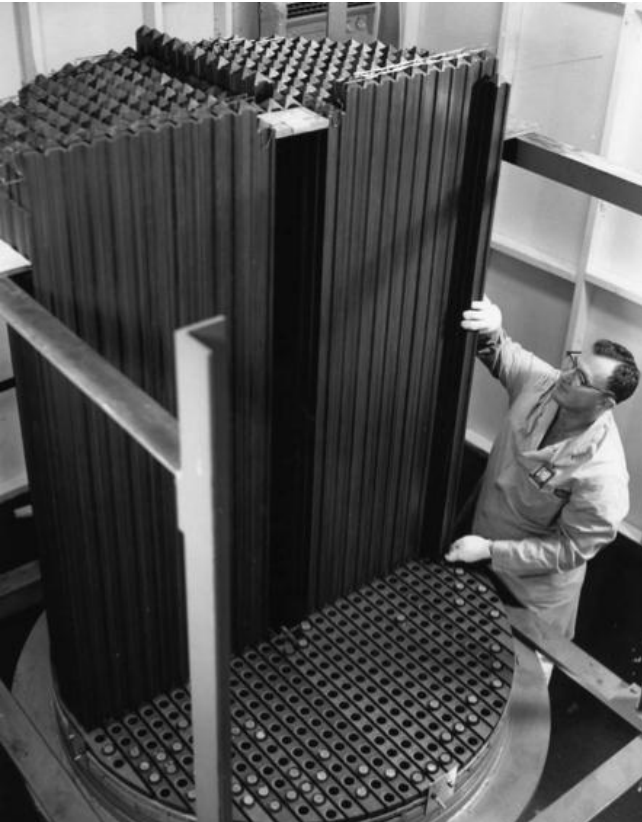
\includegraphics[height=0.7\textwidth]{./images/msre_view.png}
                \vspace*{-0.2in}
      \end{figure}
     \begin{block}{\gls{MSRE}}
       \begin{enumerate}
              \item Maximum power 8 MW$_{th}$
               \item Fuel salt
                \begin{itemize}
                   \item $^7$LiF-BeF$_2$-ZrF$_4$-UF$_4$
                   \item $^7$LiF-BeF$_2$-ZrF$_4$-UF$_4$-PuF$_3$
                \end{itemize}  
              \item First use of $^{233}$U and mixed U/Pu
              \item Single region core
              \item Operated: 1965-1969 at ORNL
              \end{enumerate}
     \end{block}
     \column[t]{5.6cm}
           \begin{figure}[t]
                \vspace*{-0.3in}
                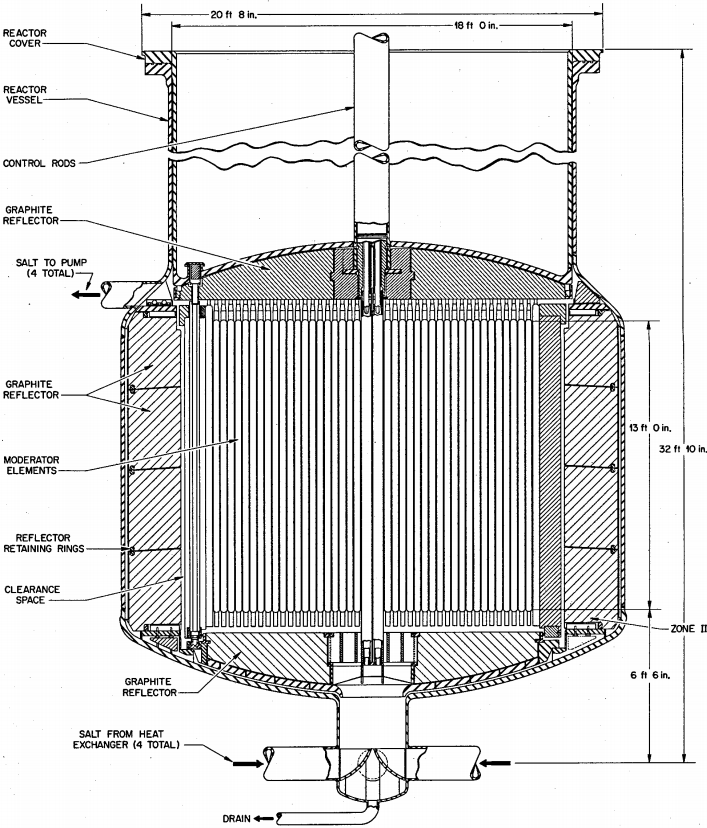
\includegraphics[height=0.7\textwidth]{./images/msbr_plain.png}
                \vspace*{-0.2in}
      \end{figure}
   \begin{block}{\glsfirst{MSBR} \cite{robertson_conceptual_1971}}
       \begin{enumerate}
       \item Maximum power 2.25GW$_{th}$, 1GW$_e$
       \item Fuel salt
         \begin{itemize}
         \item $^7$LiF-BeF$_2$-ThF$_4$-$^{233}$UF$_4$
         \item $^7$LiF-BeF$_2$-ThF$_4$-$^{233}$UF$_4$-$^{239}$PuF$_3$
         \end{itemize}  
       \item Breeding ratio 1.06
       \item Single fluid/two-region core design
      \end{enumerate}
     \end{block}
  \end{columns}
              
 \end{frame}

\subsection{Objectives}
\begin{frame}
  \frametitle{Research objectives}
                  \vspace*{-0.1in}
              \begin{block}{Goals of current study}
               \begin{enumerate}
                \item Create high-fidelity full-core 3-D model of \gls{MSBR}, ideally, without any approximations.
                \item Run steady-state criticality simulation using the SERPENT 2 Monte Carlo code \cite{leppanen_serpent_2012} 
                  to determine effective multiplication factor and neutron spectrum.
                \item Find temperature effect of reactivity varying fuel salt and graphite temperature from 900K to 1200K.
                \item Compare obtained results with Park (MCNP6) model of MSBR \cite{park_whole_2015}
                and Robertson \emph{et al.} \cite{robertson_conceptual_1971}.
               \end{enumerate}
               \end{block}
               
               \begin{block}{Why we need this model?}
               \begin{enumerate}
                \item Depletion calculations, including online reprocessing simulation.
                \item Nuclear data generation for multi-physics transient analysis (full-core model needed for asymmetric
                	accidents).
                \item Fuel cycle optimization.
               \end{enumerate}
               \end{block}

\end{frame}

\begin{frame}
  \frametitle{Input data}
  \begin{columns}
    \column[t]{6cm}
     \begin{table}[h!]
           \vspace*{-0.3in}
    \caption{Summary of principal data for \gls{MSBR} \cite{robertson_conceptual_1971}}
      \end{table}
    \begin{figure}[t]
      \vspace*{-0.45in}
            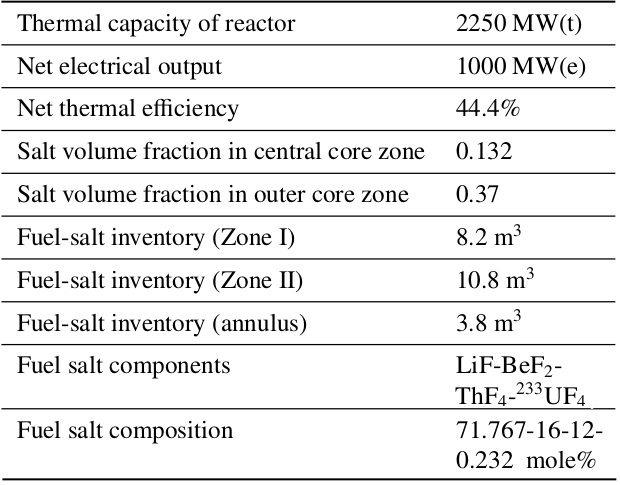
\includegraphics[height=0.55\textwidth]{./images/table_input.png}
    \end{figure}
    \begin{figure}[t]
                \vspace*{-0.2in}
                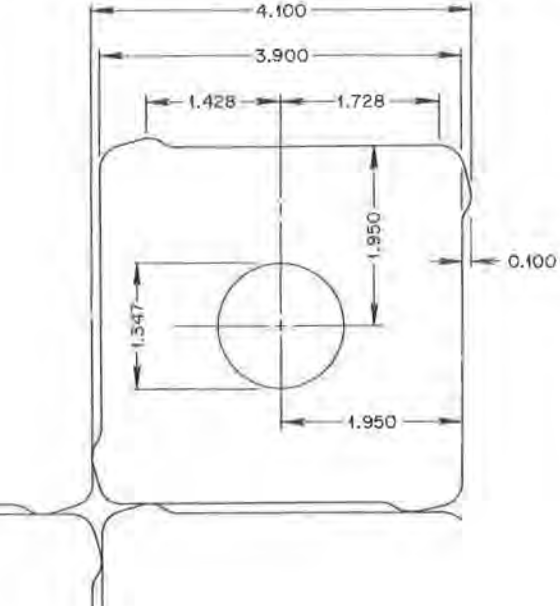
\includegraphics[height=0.55\textwidth]{./images/cell_geometry.png}
                \vspace*{-0.1in}
                \caption{Graphite moderator element.}
      \end{figure}
     \column[t]{5.6cm}
           \begin{figure}[t]
             \hspace*{-0.2in}
                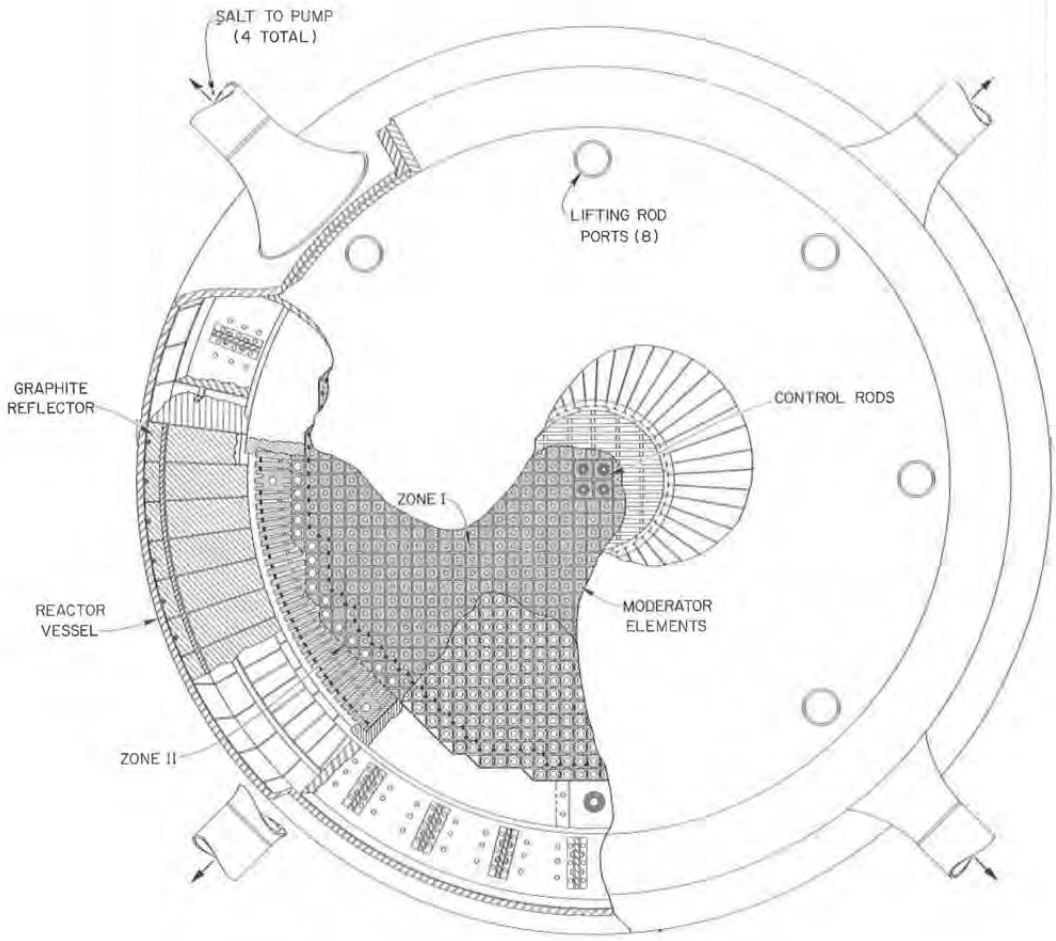
\includegraphics[height=1.0\textwidth]{./images/plan_view_vessel.png}

      \end{figure}
  \end{columns}
              
 \end{frame}
